\section{Analysis}
\label{sec:analysis}

This section analyzes \emph{why} end-to-end training yields a better sparse selector.
We first inspect the learned block selection, and find that \our covers less attention mass per layer yet its cross-layer union better matches the full attention oracle.
We then show that this more effective selection lets \our reach answers with shorter reasoning traces and fewer truncations.
Finally, we quantify the end-to-end decode efficiency and report substantial speedups over full attention.

\subsection{Analyzing the Learned Block Selection}
\label{sec:ana_selection}

\begin{figure}[!t]
    \centering

    \begin{subfigure}{0.99\linewidth}
        \centering
        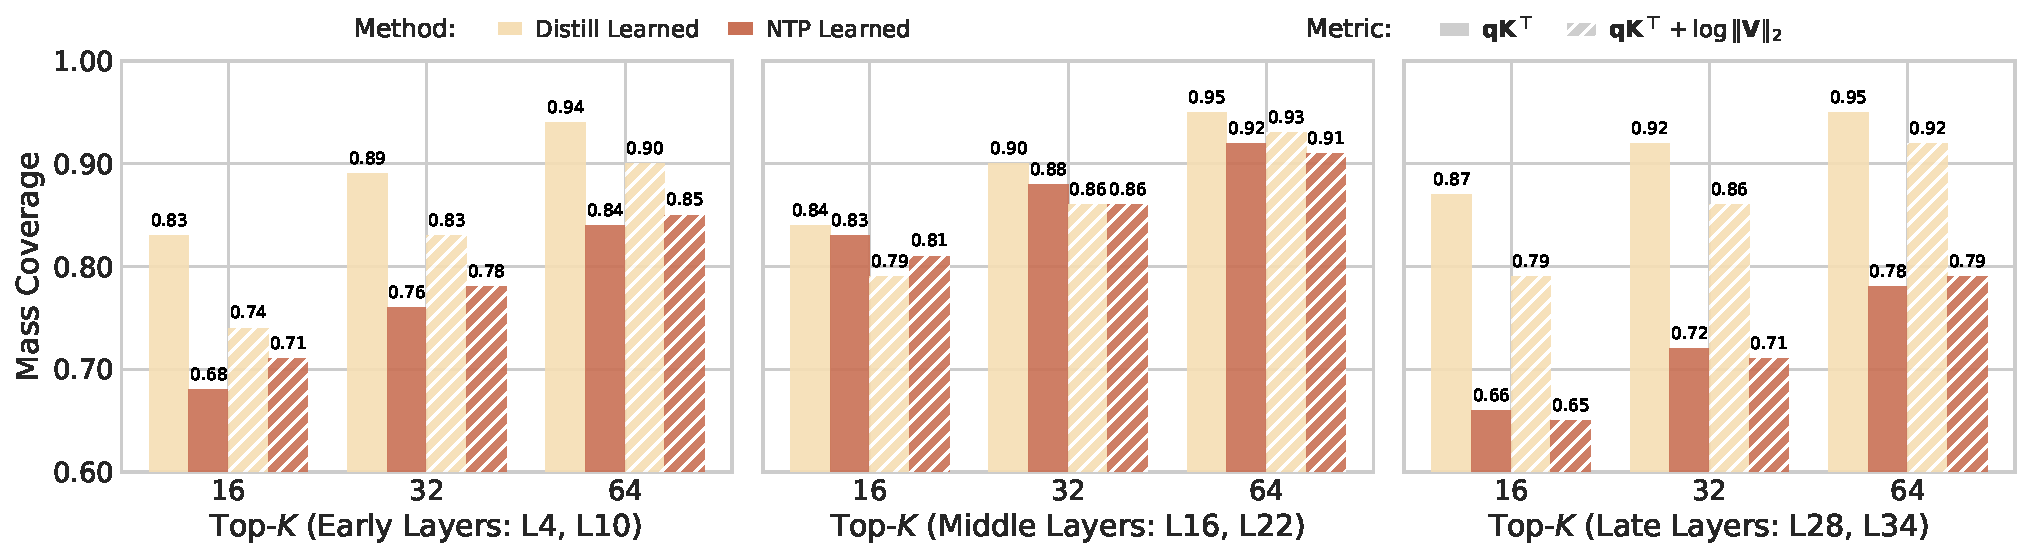
\includegraphics[width=\linewidth]{sec/fig/mass_coverage_repro.pdf}
        \caption{}
        \label{fig:mass_coverage}
    \end{subfigure}


    \begin{subfigure}{0.99\linewidth}
        \centering
        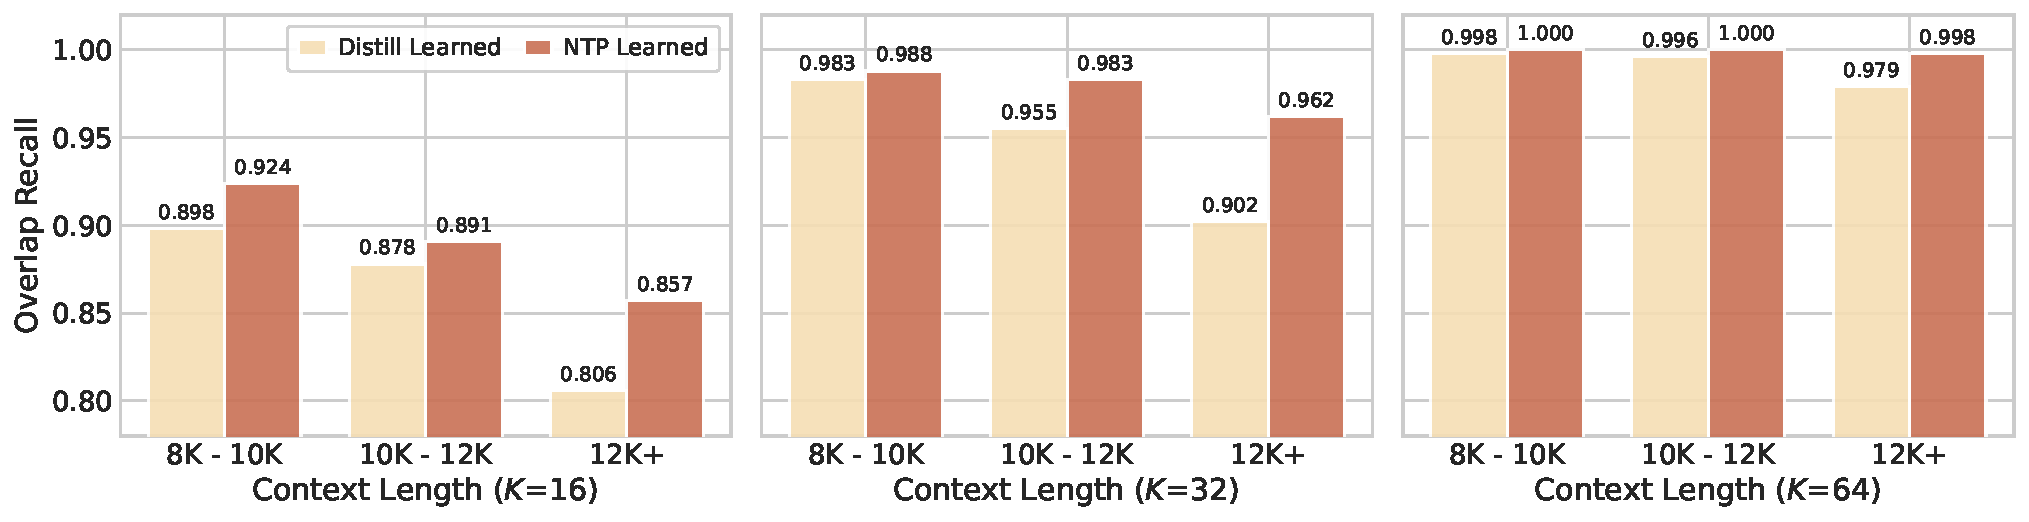
\includegraphics[width=\linewidth]{sec/fig/overlap_recall_repro.pdf}
        \caption{}
        \label{fig:overlap_recall}
    \end{subfigure}

    \caption{Analysis of the learned block selection, comparing the block selection learned by distillation (SeerAttention-R) and by end-to-end NTP (next-token prediction) training (\our).
    (a) Per-layer attention mass coverage of the selected Top-$K$ blocks, under both raw weight $\mathbf{q}\mathbf{K}^\top$, and value-aware weight $\mathbf{q}\mathbf{K}^\top+\log\|\mathbf{V}\|_2$ from STEM \cite{niu2026stemrethinkingcausalinformation}. \our covers \emph{less} mass than distillation.
    (b) Overlap recall of the cross-layer union of selected blocks against the full attention oracle. \our attains \emph{higher} recall than distillation, consistent with more complementary cross-layer selection.
    }
    \label{fig:analysis}
\end{figure}


\paragraph{Per-layer attention mass coverage.}
A natural way to assess a sparse selector is how much attention mass its selected token set $\mathcal{S}$ covers.
Reusing the attention logit $z_i=\mathbf{q}\mathbf{k}_i^\top$, we define the covered mass ratio with a per token weight $w_i$ as
\begin{equation}
    \operatorname{Cov}(\mathcal{S})
    =
    \frac{\sum_{i\in\mathcal{S}} w_i}{\sum_{j} w_j}.
    \label{eq:mass_coverage}
\end{equation}
We consider two instantiations of $w_i$. The first is $w_i=\exp(z_i)$, which depends only on the attention weight. The second is $w_i=\exp(z_i+\log\|\mathbf{v}_i\|_2)$, which additionally incorporates the magnitude of the value vector $\mathbf{v}_i$, following~\cite{niu2026stemrethinkingcausalinformation}.
As our objective is the final language modeling loss, which depends on all attention components including $\mathbf{V}$, we expect \our to favor blocks that contribute larger attention outputs.
However, \Cref{fig:mass_coverage} shows that \our covers \emph{less} mass than distillation under both metrics in almost all layers.
One possible explanation is that distillation explicitly optimizes for full attention coverage as its training target, naturally encouraging higher attention mass coverage, whereas \our is never trained to match the full attention distribution.

\paragraph{Overlap with the full attention oracle.}
The per-layer coverage above, however, ignores that selection is distributed across layers: a block missed at one layer can still be attended at another.
We therefore take, for each method, the union of its selected blocks across all layers and measure how much of the full attention model's attended blocks it recovers.
On long training sequences ($>$8K) with Qwen3-4B, we obtain the oracle set from full attention; since it uses GQA, we aggregate the per-head Top-$K$ within each group into one group-level set by majority vote.
Taking the union of these sets over all $L$ layers gives the oracle set $\mathcal{I}_{\text{all}}^{\star}$, and applying the same procedure to a method's own selection gives $\mathcal{I}_{\text{all}}$.
We then report the overlap recall
\begin{equation}
    \operatorname{Recall}(\mathcal{I}_{\text{all}}, \mathcal{I}_{\text{all}}^{\star})
    =
    \frac{|\mathcal{I}_{\text{all}}\cap\mathcal{I}_{\text{all}}^{\star}|}{|\mathcal{I}_{\text{all}}^{\star}|},
    \qquad
    \mathcal{I}_{\text{all}}=\bigcup_{j=1}^{L}\mathcal{I}_{j},
    \label{eq:overlap_recall}
\end{equation}
where $\mathcal{I}_{j}$ is the per-layer block set at layer $j$ and $\mathcal{I}_{\text{all}}^{\star}$ is defined analogously.
As shown in \Cref{fig:overlap_recall}, \our attains consistently higher overlap recall across context lengths and budgets.
This matches our expectation: distillation fits the full attention layer by layer as a local objective, whereas \our is trained end-to-end, so its block selection is optimized jointly across layers.
As a result, even though \our retains less attention mass within each individual layer, its per-layer choices are more complementary, and their union attains higher overlap recall against the oracle.


\subsection{Analyzing the Generation Behavior}
\label{sec:ana_token}

\begin{figure}[!t]
    \centering
    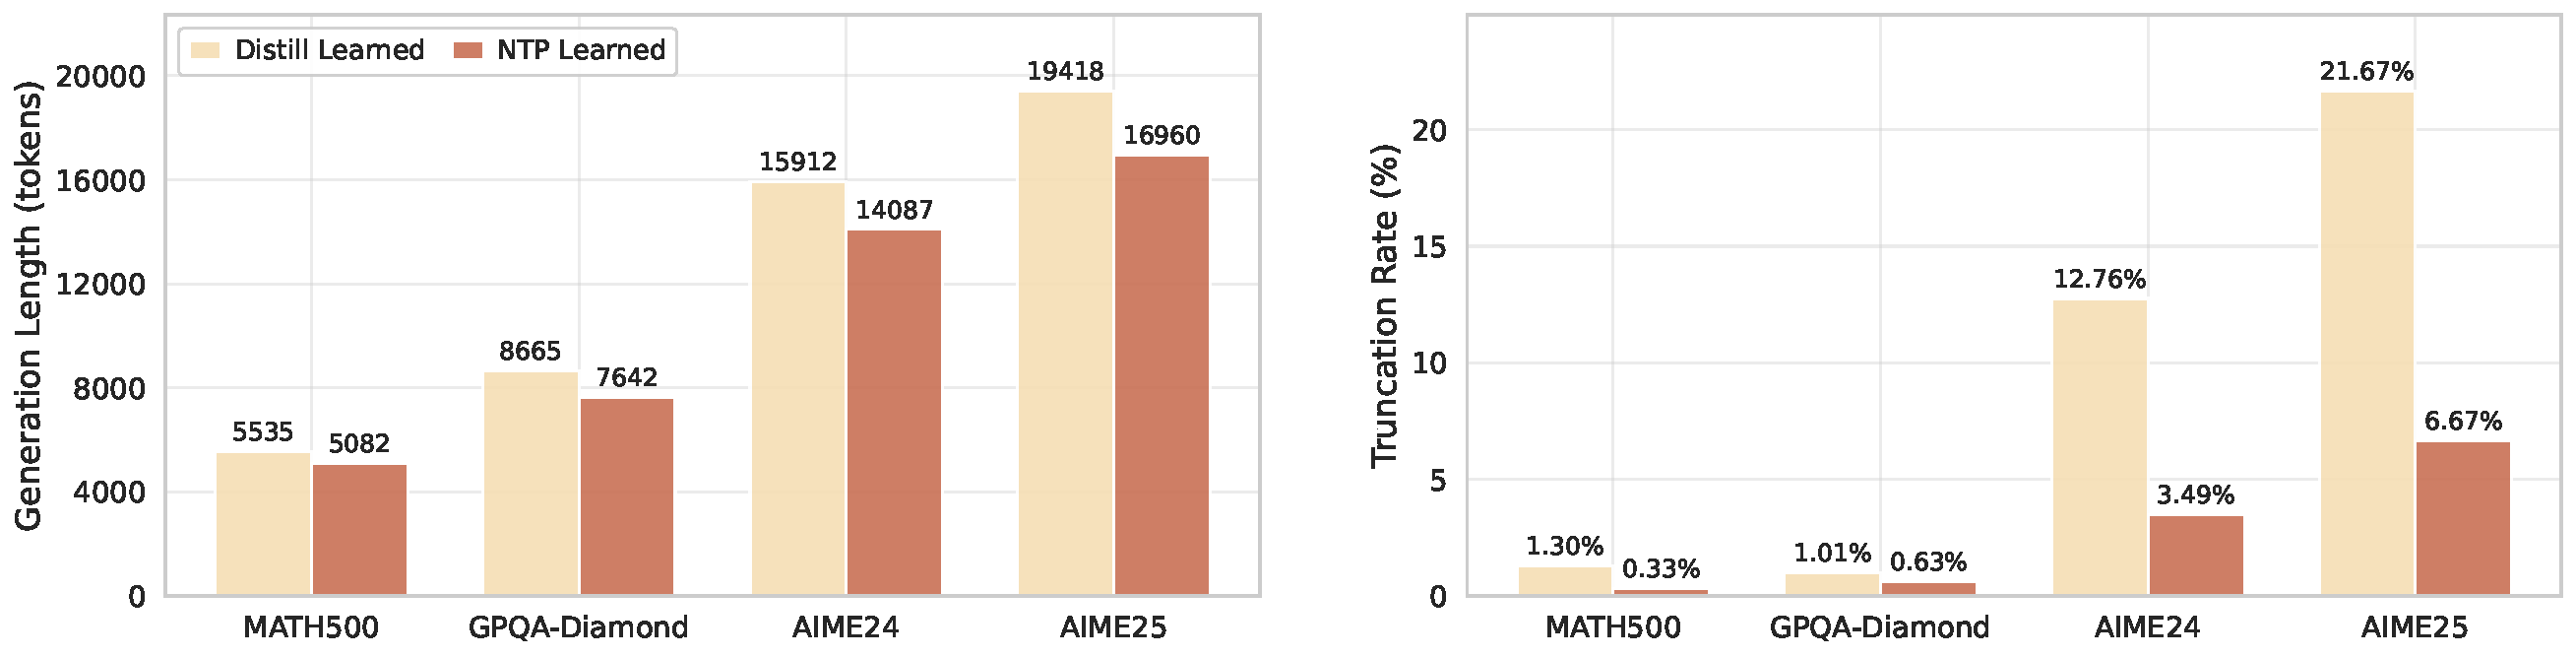
\includegraphics[width=0.99\linewidth]{sec/fig/gate_compare_len_trunc.pdf}
    \caption{Generation behavior of distillation (SeerAttention-R) and end-to-end NTP (\our) on Qwen3-4B at a 4096 token budget across four reasoning benchmarks. Left: average generation length; \our generates shorter traces.
    Right: truncation rate under a maximum generation length of 32{,}768; \our truncates less often. These trends are consistent with more effective context selection, suggesting \our reaches answers with fewer tokens, with the gap largest on the harder AIME tasks.}
    \label{fig:token_eff}
\end{figure}

Beyond final accuracy, the quality of sparse selection also affects token efficiency, measured here by the generation length needed to reach an answer.
When important context is dropped, the model tends to generate longer, less focused reasoning traces and is more likely to hit the maximum generation length before finishing.
We therefore compare SeerAttention-R and \our on Qwen3-4B at a 4096 token budget, reporting the average generation length and the truncation rate under a maximum length of 32{,}768 (\Cref{fig:token_eff}).
Across all four reasoning benchmarks, \our produces shorter generations and a lower truncation rate, with the gap widening on the harder AIME tasks where long reasoning is required.
These results are consistent with more effective context selection: they suggest that \our can complete its reasoning with fewer tokens and less frequent truncation, complementing the accuracy gains in Section~\ref{sec:exp_posttrain}.


\subsection{End-to-End Decode Efficiency}
\label{sec:e2e_efficiency}

\begin{figure}[!t]
    \centering

    \begin{subfigure}{0.33\linewidth}
        \centering
        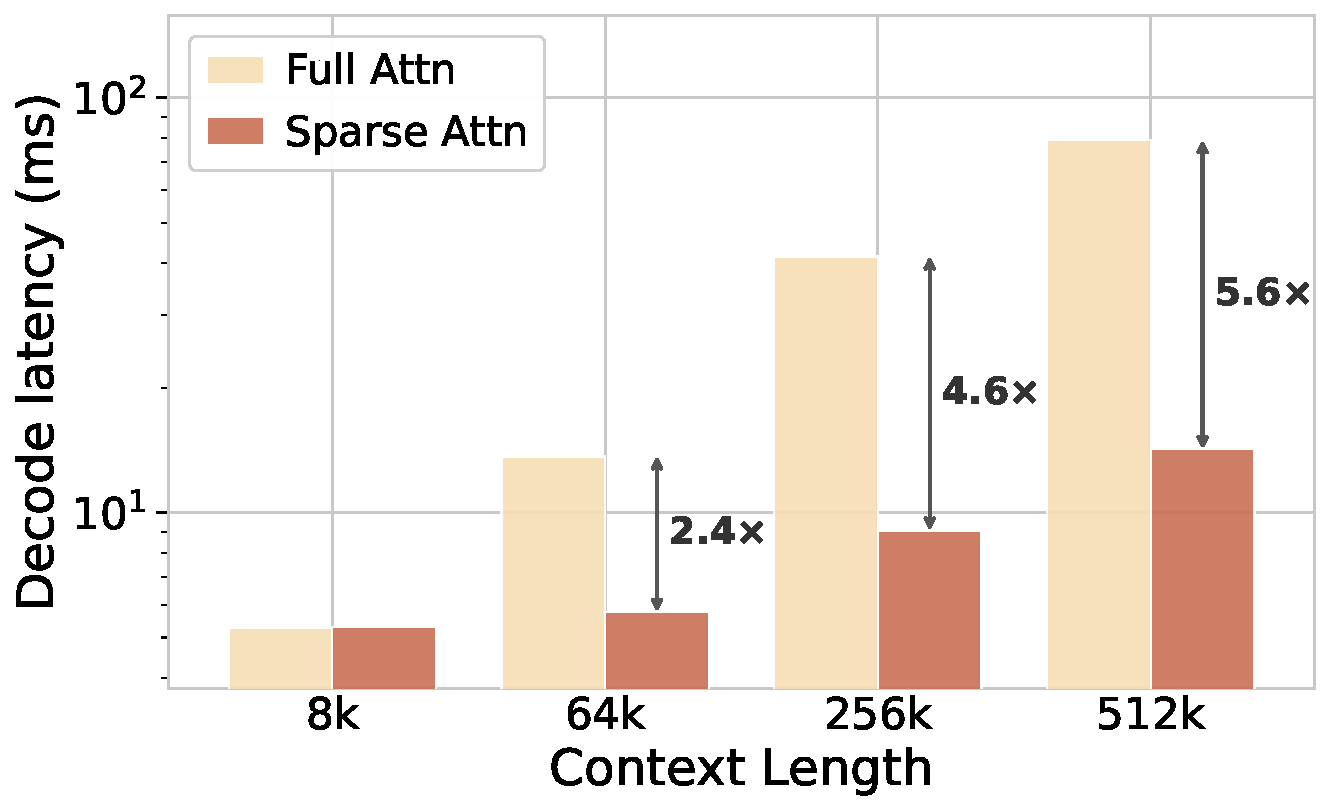
\includegraphics[width=\linewidth]{sec/fig/taskA_speedup.pdf}
        \caption{}
        \label{fig:e2e_latency}
    \end{subfigure}\hfill
    \begin{subfigure}{0.33\linewidth}
        \centering
        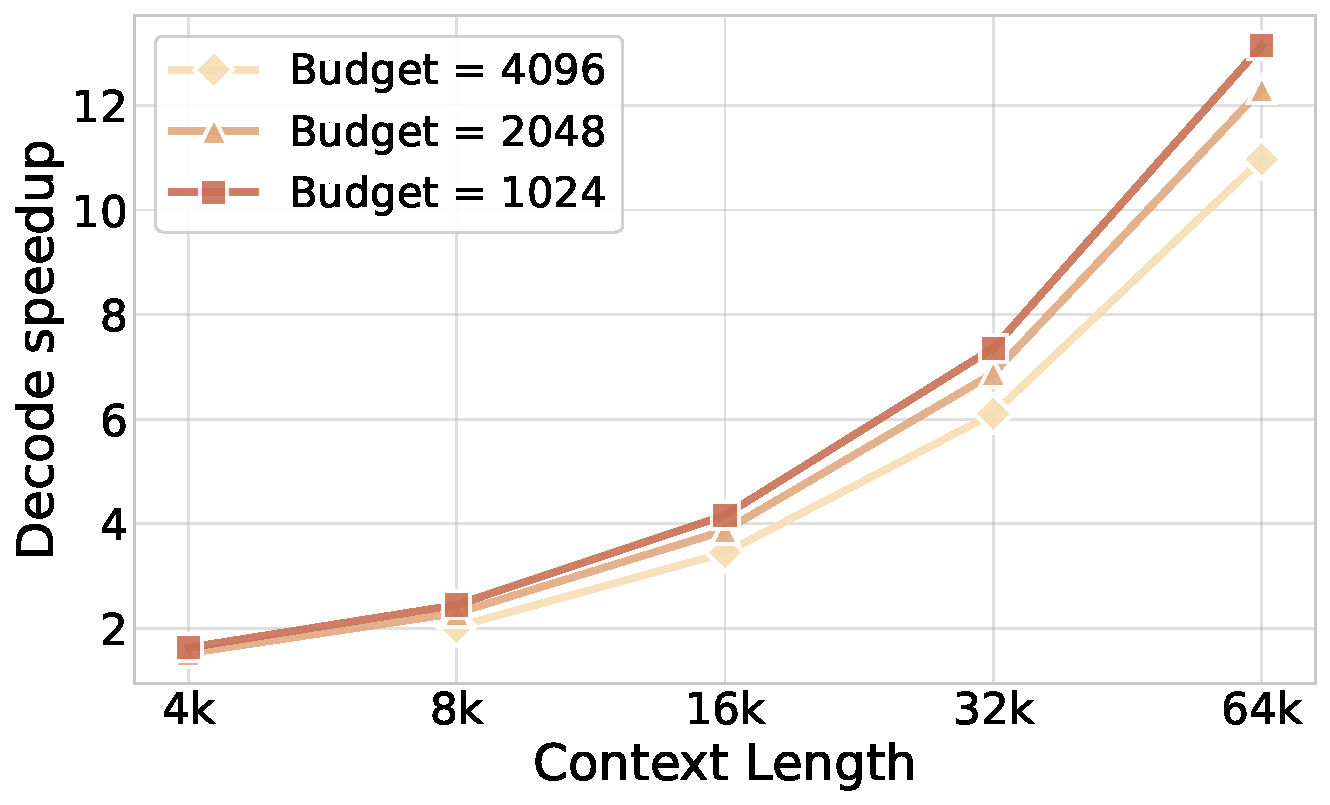
\includegraphics[width=\linewidth]{sec/fig/taskB_budget_sweep.pdf}
        \caption{}
        \label{fig:e2e_budget}
    \end{subfigure}\hfill
    \begin{subfigure}{0.33\linewidth}
        \centering
        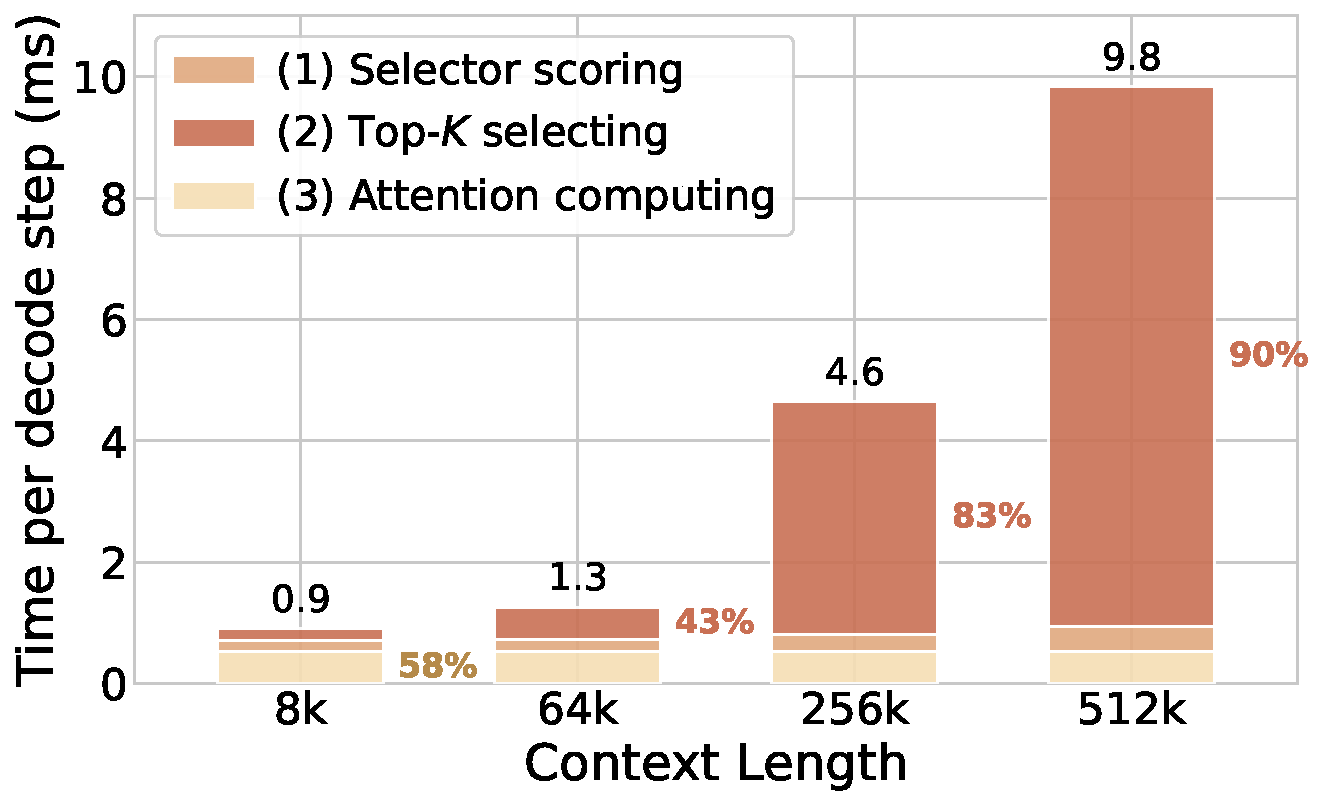
\includegraphics[width=\linewidth]{sec/fig/taskC_attn_breakdown.pdf}
        \caption{}
        \label{fig:e2e_breakdown}
    \end{subfigure}

    \caption{
    End-to-end decode efficiency of \our versus dense attention on Qwen3-4B in SGLang (single GPU, CUDA graphs, steady-state decode).
    (a) At batch 1, dense latency grows linearly with context length, while \our remains nearly constant, achieving up to 5.6$\times$ lower latency at 512K.
    (b) At batch 8, speedup reaches $\sim$13$\times$ and is largely insensitive to the token budget.
    (c) Sparse-decode latency breakdown: attention cost remains constant, while Top-$K$ selection dominates at long contexts.
    }
    \label{fig:e2e_efficiency}
\end{figure}


\paragraph{Decode speedup over full attention.}
We measure wall-clock decode efficiency by serving Qwen3-4B in SGLang with
our block sparse attention against full attention under an identical
configuration: a single GPU (tensor parallel size 1), CUDA graphs enabled,
chunked prefill, and a steady-state decode measurement (the input is prefilled,
then 512 generated tokens are timed).
Since \our sparsifies \emph{decode-time} attention only, prefill is unchanged,
and the reported numbers isolate the per-token decode cost.
Full attention must read the entire KV cache at every step, so its decode
latency grows linearly with context length, whereas \our reads only a fixed
token budget of blocks and stays essentially flat.
The gap therefore widens with context: at batch 1
(\Cref{fig:e2e_latency}) the two are near parity at 8K but \our is
2.4$\times$, 4.6$\times$, and 5.6$\times$ faster at 64K, 256K, and 512K.
Increasing the batch amortizes the fixed per-step overhead and further favors
sparsity: at batch 8 (\Cref{fig:e2e_budget}) the speedup reaches
$\sim$13$\times$ at 64K.
A tighter token budget reads fewer blocks and is thus faster, but the difference
across budgets is modest, indicating that the benefit
comes primarily from avoiding the full KV read rather than from the exact budget.

\paragraph{Decode step cost breakdown.}
To understand the scaling behavior, we decompose one sparse attention decode
step into its three components: selector scoring (the gate query projection and
its dot-product against the block summaries), Top-$K$ block selection, and the
attention compute over the selected blocks (\Cref{fig:e2e_breakdown}).
The attention compute is context invariant, since the number of blocks read is
capped by the token budget regardless of sequence length.
Selector scoring, by contrast, scans all block summaries and thus grows with
context in absolute terms, rising from well below the attention compute at 8K
to roughly matching it at 512K; extrapolating to longer context, it is
expected to surpass the attention compute.
The Top-$K$ selection grows even faster, as it must rank all candidate blocks,
and comes to dominate the step, shifting from 21$\%$ at 8K
(where attention compute dominates at 58$\%$) to 90$\%$ at 512K.
This identifies the selection stage, Top-$K$ ranking together with the growing
selector scoring, rather than the attention compute, as the primary bottleneck
and the main target for further kernel optimization at very long context.
